% Plan:
%
% Spis treści
% Spis rysunków
% Słowniczek skrótów
%
% Wstęp (1-2 strony): geneza, obszar, zawartość, dokonania autorów, opis struktury pracy
%
% Rozdziały merytoryczne (4-5, zrównoważone objętościowo):
%   Preambuła (ok. 0.5 strony)
%   Punkty merytoryczne (4-6)
%   Podsumowanie rozdziału
%
%   * opis technologii i uzasadnienie wyboru do rozwiązania problemu
%   * analiza wymagań + projekt systemu (architektura)
%   * opis implementacji, sposób uruchomienia
%   * badania eksperymentalne (tutaj także: profiling, opóźnienia)
%
% Podsumowanie pracy / Zakończenie
%   Wnioski końcowe
%   Co się udało / nie udało (+dlaczego!)
%   Możliwości rozwoju
%
% Spis literatury (numerowany, w tekście _muszą_ być odniesienia, ~20 pozycji)
%
%
% INNE:
%   * całość - ok. 60-70 stron
%   * numeracja - nie więcej, niż 3-poziomowa


\documentclass[11pt]{book}
\usepackage[top=3cm, bottom=4cm]{geometry}
\usepackage[usenames,dvipsnames]{color}


% \usepackage[polish]{babel}
\usepackage[utf8]{inputenc}
\usepackage[T1]{fontenc}
\usepackage{fullpage}
\usepackage[pdfborder={0 0 0}]{hyperref}
\usepackage{float}
\usepackage{graphicx}
\usepackage{scrtime}
\usepackage{tabularx}
\usepackage{listings} 
\usepackage{caption}
\usepackage{color}
\usepackage{hyperref}
\usepackage{tikz}
% \usepackage[toc,acronym]{glossaries}
\usetikzlibrary{positioning,chains,backgrounds,fit,scopes}
% \usetikzlibrary{chains}

\newcommand{\code}[1]{\begin{tt}{#1}\end{tt}}

\newcommand{\reqlabel}[1]{{\textcolor{Red}{\textbf{#1}}\label{#1}}}
\newcommand{\reqref}[1]{\hyperref[#1]{{\textcolor{Red}{\textbf{#1}}}}}

\newcommand{\tasklabel}[1]{{\textcolor{Blue}{\textbf{#1}}\label{#1}}}
\newcommand{\taskref}[1]{\hyperref[#1]{{\textcolor{Blue}{\textbf{#1}}}}}

% include TikZ styles
\tikzstyle{terminal}=[
  rectangle,
  minimum size=6mm, rounded corners=3mm,
  very thick,
  draw=black!50,
  top color=white,bottom color=black!20,
  font=\ttfamily
]




\title{Component-based system for management of multilevel virtualization of networking resources}
\author{Robert Boczek \and Dawid Ciepliński}

\begin{document}

  \maketitle
    
  \tableofcontents

  % TODO podzial pracy

  \chapter{Introduction}

    % QoS, rezerwacja zasobów, izolacja we współczesnych systemach informatycznych


  \chapter{Context}  % TODO ładniej

    \section*{Chapter overview}


    \section{QoS-aware networking}

      % IntServ, DiffServ, inne


    \section{Resource virtualization approaches}

      % TODO classify and define virtualization types


    \section{Multilevel network virtualization}

      \subsection{Virtual network resources}

      \subsection{Fine-grained QoS control}

      \subsection{Virtual appliances}

      \subsection{,,Network in a box'' concept}


    \section{Applications and benefits of virtual infrastructures}

      \subsection{Testing and simulations}

      \subsection{Improving server-side infrastructure scalability}

      \subsection{Infrastructure as a service}

      \subsection{The role of resource virtualization in the SOA stack}


    \section*{Summary}


  \chapter{Requirements analysis}
    
    \section*{Chapter overview}

    \section{Functional requirements}

      \subsection{Instantiation}

      \subsection{Discovery}

      \subsection{Accounting}  % kz: raczej Monitoring


    \section{Non-functional requirements}

    \section{Underlying environment characteristics}

    \section{General approach and problems it imposes}

      \subsection{Load balancing / Deployment}

      \subsection{Infrastructure isolation}

      \subsection{Broadcast domain preservation}

      \subsection{Constraints}


    \section*{Summary}


  \chapter{Solaris OS as a resource virtualization environment}
  
    %TODO change chapter title !!!
    % TODO  actually, Solaris 10, Solaris 11 and OpenSolaris are described here!

    The chapter provides an overview of Oracle Solaris operating system and evaluates it as a platform for resource
    virtualization. The chapter describes Solaris 11 Express release of the system, as it is the first release
    (together with OpenSolaris) with Crossbow technology integrated. Special emphasis is put on the networking-related
    aspects of virtualization. Thus, the Solaris Crossbow technology is described in detail.

    Section \ref{sec:sol:general} contains introductory information about the system. A short historical note is
    presented and general description follows. Main components of the system are introduced and described.
    
    Each of the remaining sections describe in more detail these parts of the operating system that are extensively
    used by the implemented system. Section \ref{sec:sol:containers} investigates the Solaris Zones technology. After
    defining the concept of zones, zone lifecycle model is presented, the achieved level of process isolation is
    described and discussion of Zones advantages in comparison to non-virtualized environments follows.

    Section \ref{sec:sol:xbow} introduces Solaris Crossbow - lightweight network virtualization environment. The
    section starts with general description of the technology. Next, components crucial to efficiency improvement are
    presented in detail. Etherstubs, VNICs and flows are described. These are building blocks used to create
    virtualized network elements and apply QoS policies. The section ends with the comparison between Crossbow and
    DiffServ and a method of integration of these two solutions is presented.

    Section \ref{sec:sol:res} provides an overview of resource control methods offered by the Solaris OS. The types
    of resource management mechanisms (constraints, partitioning and scheduling) are identified and defined. Resource
    control hierarchy used by the system is depicted and explained. Also, the accounting facility is described. The
    types of resources extended accounting can work with are enumerated and examples of data that can be gathered are
    listed.


    \section{General information}
    \label{sec:sol:general}

      Oracle Solaris is a \textit{multiuser, multitasking, multithreading UNIX-like operating system} \cite{reference}.
      Since its release in 1992 (as Sun Solaris 1), the system became one of the most popular environments supporting
      enterprise software. Nowadays, big corporations and companies as well as individual developers use it to do their
      business and deliver reliable and scalable services.

      The Solaris OS provides unique set of tools that support virtualization of practically all types of resources at
      various levels. There is Logical Domains (LDOMs) technology for full virtualization and lightweight Zones, when
      all that is needed is the isolation of processes. Logical domains can be connected with complex virtual networks
      that are created with virtual switches (vsw) and virtual network devices (vnet) \cite{ldomag} and Crossbow can be
      used to enable lightweight and efficient networking for zones, exploiting capabilities of underlying hardware
      layer (network interface cards with virtualization level 1, 2 or 3 \cite{santos}).

      Resource utilization can be managed with integrated administration tools. Resource access policies can be created
      with high level of granularity (per-process resource control) as well as in more general way (limiting resource
      access for LDOMs). Resource consumption can be subject of monitoring and accounting. With extended accounting
      subsystem enabled, it is possible to capture detailed accounting data even for single processes. Gathered data
      include CPU usage, number of bytes received or transmitted per DiffServ or Crossbow flow and more.

      As far as multiple physical machines are considered, there is also support for VLANs (Virtual Local Area Network).
      Thanks to VLAN tagging support, it is possible to build systems that guarantee the quality of service from the
      lowest levels up, even for services belonging to different systems and consolidated within single physical machine.

      \begin{figure}[H]
        % TODO expand
        \begin{center}
          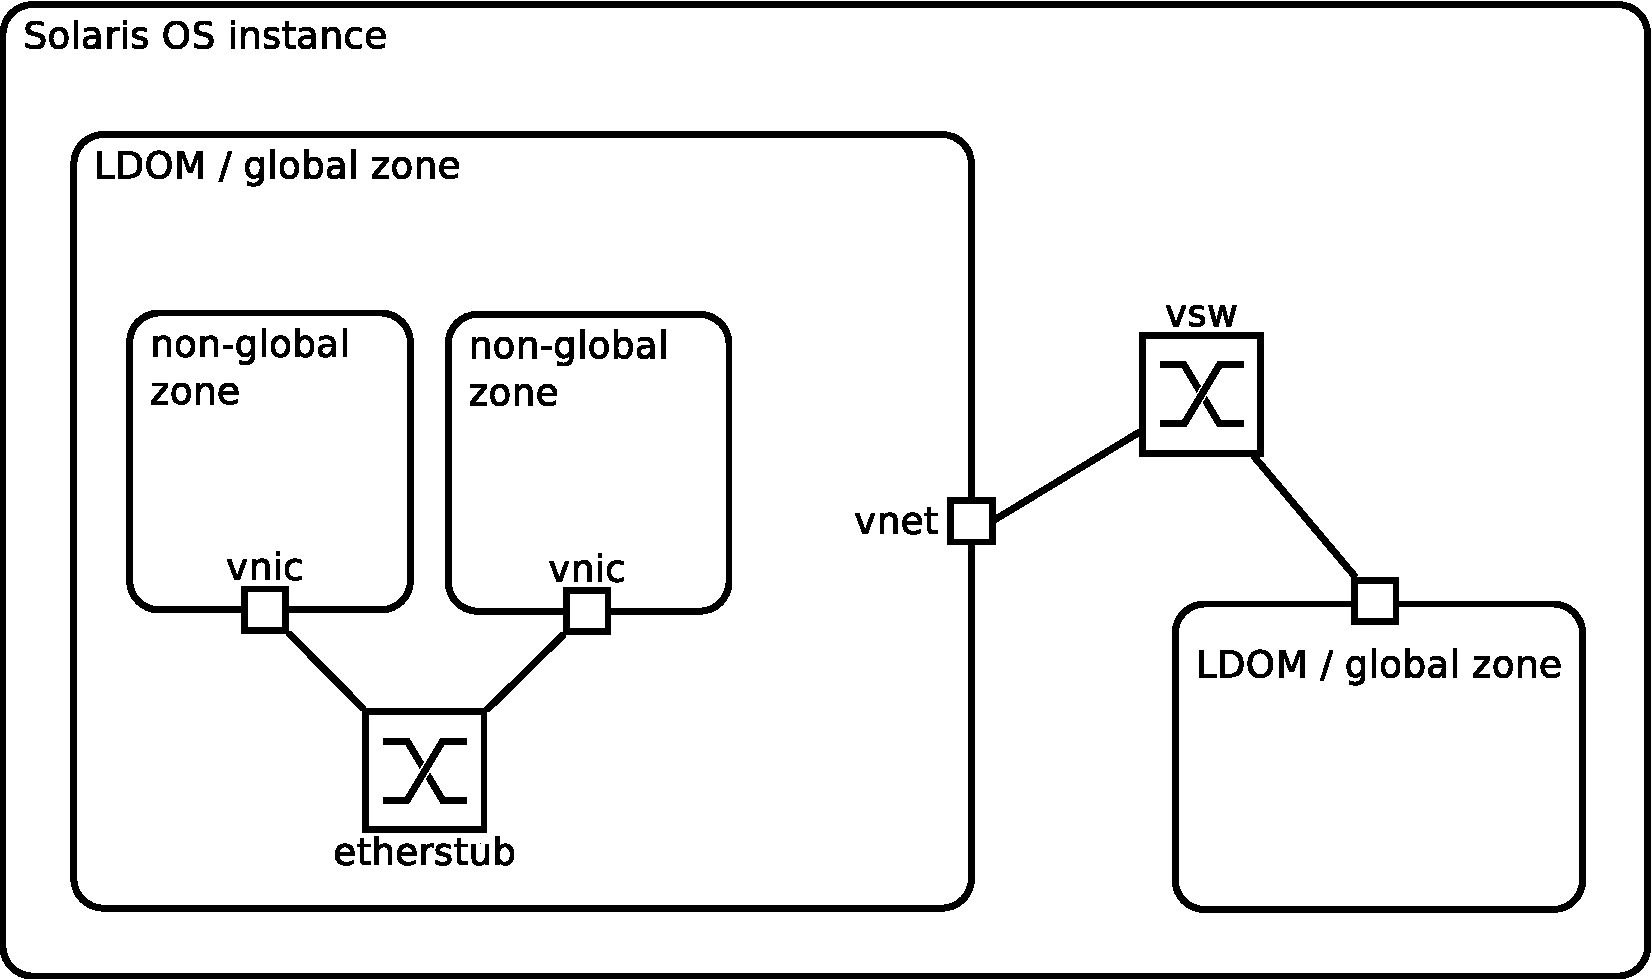
\includegraphics[width=.7\textwidth]{img/solaris/full-featured.pdf}
        \end{center}

        \caption{The variety of resources that can be virtualized with Solaris OS}
      \end{figure}

      As it can be seen, the Solaris operating system is accompanied by vast variety of virtualization-supporting
      subsystems. This multiplicity and flexibility makes it a promising platform for service provisioning and building
      even more abstract architectures on top of it. The following sections describe selected aspects of the system in
      more detail.


    \section{OS-level virtualization with Solaris Containers}
    \label{sec:sol:containers}

      % TODO citation for WPARs

      The concept of lightweight (OS-level) virtualization is supported by most modern operating systems. The solutions
      are either integrated into the system's kernel and accessible as soon as it is installed (Solaris Containers, AIX
      Workload partitions, BSD jails \cite{kamp}) or are provided by third-party manufacturers as kernel patches and
      utility software (OpenVZ and LXC for Linux OS). Because of awareness of other system components and integration 
      with them, it can be expected that Zones have more potential than other virtualization methods.


      \subsection{General information}
      \label{sub:}

        Zones technology was introduced as of Solaris OS 10. It provides a way of partitioning system resources and
        allows for isolated and secure application execution environment \cite{sag}. Solaris Zones, together with
        resource management functionality, constitute the Solaris Container environment.

        There are two types of zones: global and non-global. Global zone is the default one and is used to execute
        applications as well as to administer the system. Non-global zones can be created from within the global zone
        only. A single operating system instance with one global zone can host as many as 8192 non-global zones
        \cite{sag}.

        Zones can be assigned system resources such as CPU capacity, the amount of random-access memory or even maximum
        number of lightweight processes that can be running simultaneously. Also, network isolation is supported at two
        levels: basic, at the IP layer, and network isolation and advanced virtualization with fine grained quality of
        service control using the Crossbow technology.

        Each zone can run a different set of applications, with optional translation of system calls (Branded Zones
        Technology) thus emulating different operating environments \cite{sag}. The user is able to create a branded
        zone with translation of Linux system calls and run Linux-specific applications without code recompilation.

        \begin{figure}[H]
          \begin{center}
            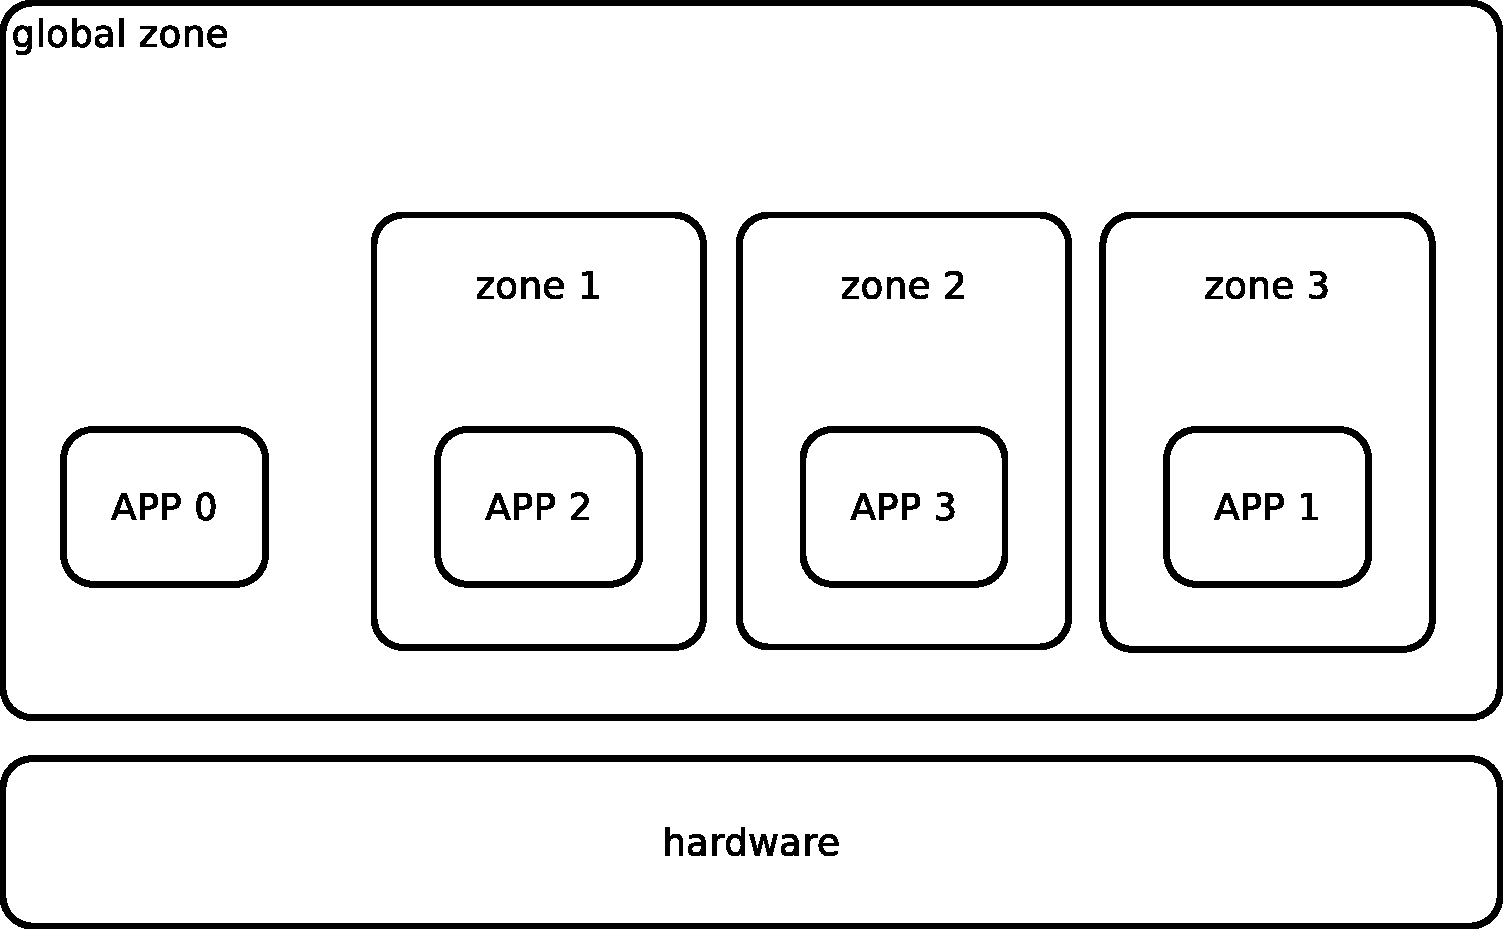
\includegraphics[width=0.7\textwidth]{img/solaris/zones-high-level.pdf}
          \end{center}

          \caption{Solaris Zones high-level view}
        \end{figure}


      \subsection{Zone lifecycle}
      \label{sub:}

        A model was created to describe the states in which each zone must exist and its possible transitions. A non-global zone can be
        in one of six states: \textit{configured}, \textit{incomplete}, \textit{installed}, \textit{ready},
        \textit{running}, \textit{shutting down or down} \cite{sag}. Figure \ref{fig:sol:lifecycle} depicts the model.

        \begin{figure}[H]
          \begin{center}
            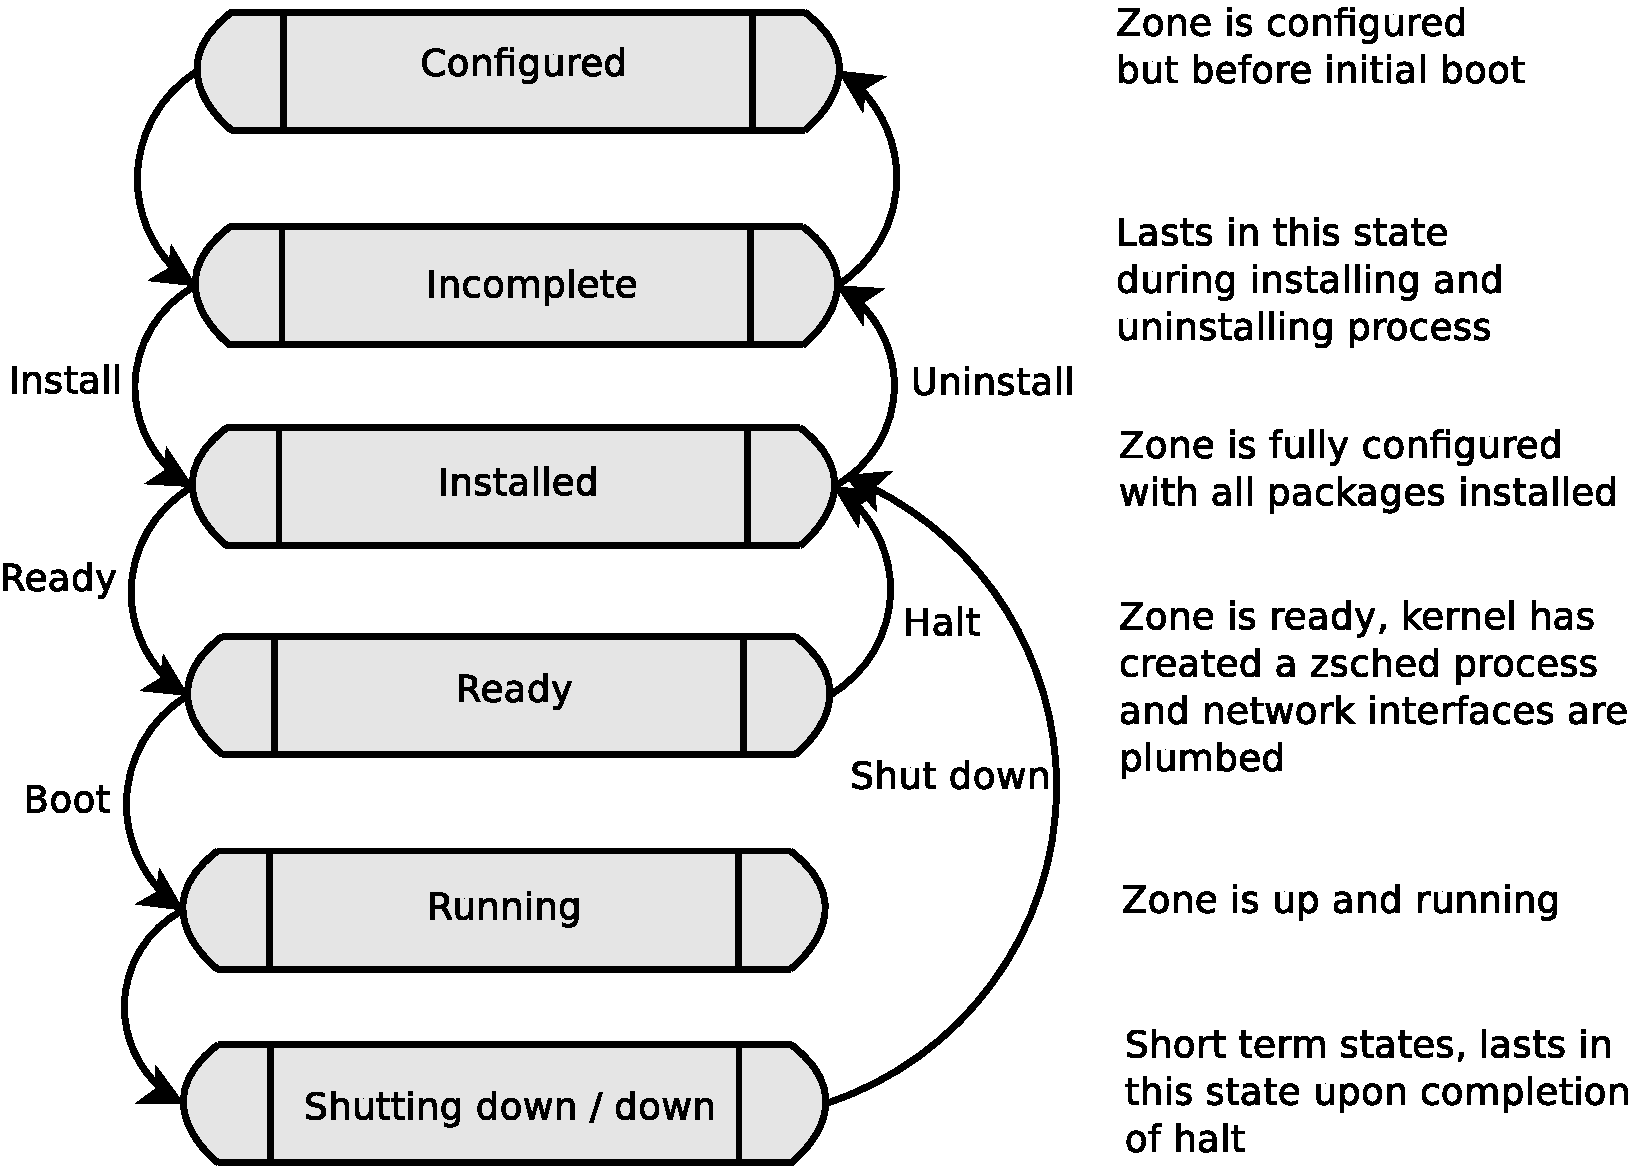
\includegraphics[width=0.7\textwidth]{img/solaris/zone_states.pdf}
          \end{center}

          \caption{Zone states and possible transitions}
          \label{fig:sol:lifecycle}
        \end{figure}


      \subsection{Isolation of processes}
      \label{sub:}

        The Containers environment offers a high level of application security and isolation. This is accomplished by
        imposing software bounds on the resource usage and introduction of additional abstraction layer over hardware.

        Every process and its children are bound to concrete zone and the assignment cannot be changed. Moreover, it is
        impossible for processes in distinct zones to monitor each other operation. They are not visible to each other
        and no interprocess communication can take place, except for network-based one, if enabled by the administrator.

        Because of the isolation, an application failure possibly affects only the processes in the containing zone.
        Assuming no interaction between processes in separate zones, the rest of the system remains intact and can
        operate normally.
        
        % TODO easier recovery, independent container management
      

      \subsection{Advantages of Containers technology when compared to non-virtualized environments}
      \label{sub:}

        The architecture of Solaris Containers makes it a competitive solution as far as systems administration and
        operation efficiency is concerned. The technology, imposing negligible overhead \cite{price}, allows to perform
        tasks that would be impossible or very hard to accomplish if traditional setup is used. Examples of such tasks
        include dynamic resource assignment, instantaneous cloning and migration of systems between physical nodes.

        The technology allows for running a number of isolated instances of operating system sharing CPU time,
        physical network bandwidth, filesystem contents and binary code. Sharing of these resources can greatly improve
        overall system efficiency and reduce the amount of occupied memory. The speed of network communication between
        different zones can also be improved thanks to ,,short-circuited'' traffic (i.e. omitting the layers below IP in
        the OSI/ISO stack). The instances are able to execute applications with minimum overhead introduced mainly due
        to accessing commands and libraries through the lofs (loopback filesystem) \cite{price,fsag}.

        When using file system that supports snapshots (as, for example, ZFS), zones can be
        serialized (a snapshot of the file system can be taken) and sent over the network connection or other means of
        data transfer to another machine. There, the zone can be restored and operate as a part of the host system.

        Another important aspect of building the infrastructure with containers is resource control. The Solaris system
        makes it possible to define resource controls (rctls) at various levels, also on per-zone basis. CPU shares,
        maximum number of lightweight processes and maximum swap size are examples of resource control properties that
        can be set for a zone. This can be further extended by providing fine-grained properties at project, task and
        process levels \cite{sag}. The resource control process is dynamic - assignments can be changed as the system
        is running, without interrupting the container's normal operation. This can be of extreme importance as far
        as high-availability systems are considered.

        Containers facilitate service consolidation - all components of a system can be executed in a single machine
        with network-based communication handled entirely by the host operating system, thus eliminating the need for
        additional networking hardware and its management. The consolidated infrastructure becomes more flexible as the
        majority of administration tasks can be performed by issuing a series of terminal commands. All these factors
        make total cost of ownership lower \cite{price}.

        \begin{figure}[H]
          \begin{center}
            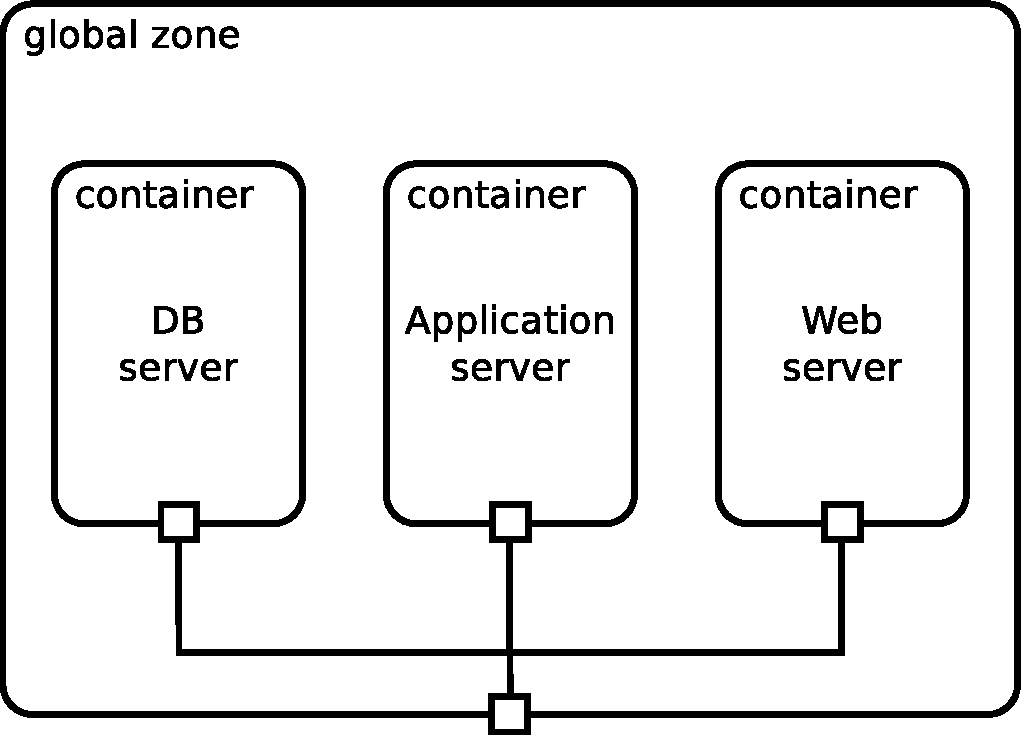
\includegraphics[width=.6\textwidth]{img/solaris/consolidation.pdf}
          \end{center}

          \caption{Service consolidation within a Solaris OS instance with internal network connectivity}
        \end{figure}


      \subsection{Virtual appliances}
      \label{sub:}

        Virtual appliance is a \textit{pre-built, pre-configured, ready-to-run (enterprise) application packaged along
        with an optimized operating system inside a virtual machine} \cite{changhua}. Solaris Zones, together with other
        components of the Solaris OS, constitute a complete framework that implements virtual appliance approach to
        systems management.

        The main problem virtual appliances can solve is the complexity and duration of application deployment process.
        In general, a service deployment can be described as comprising the following stages: preparation (learning the
        dependencies), pre-installation, installation and post-installation. With traditional (non-virtualized)
        approach, these stages have to be repeated every time a service is deployed on different machines.

        \begin{figure}[H]
          \begin{center}
            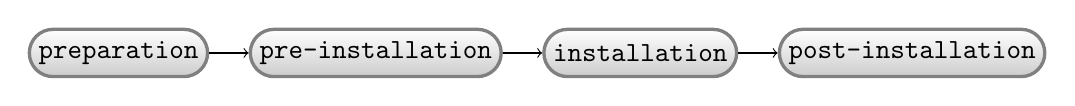
\begin{tikzpicture}[start chain,
                                node distance=5mm,
                                every node/.style={on chain, join, terminal},
                                every join/.style={->}]

              \node {preparation};
              \node {pre-installation};
              \node {installation};
              \node {post-installation};
            \end{tikzpicture}
          \end{center}

          \caption{Traditional application deployment stages.}
        \end{figure}

        % TODO verify the stages

        Virtual appliance approach makes it possible to reduce deployment time significantly \cite{changhua}. This is
        achieved by performing most of the deployment stages once and storing the configured environment in a virtual
        appliance. The appliance can then be moved to publicly-available repository for actual deployment on host
        systems.

        \begin{figure}[H]
          \begin{center}
            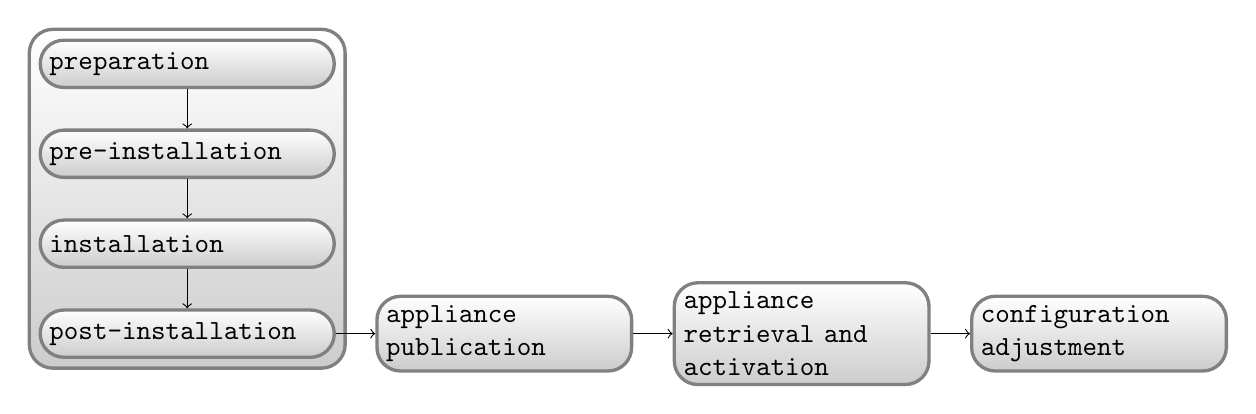
\begin{tikzpicture}[node distance=5mm,]

              { [start chain, every node/.style={terminal, on chain, join, text width=3cm}, every join/.style={->}]

                { [every on chain/.style={text width=3.5cm}]

                  \node (prep)                 {preparation};
                  \node (pre)  [below=of prep] {pre-installation};
                  \node (ins)  [below=of pre]  {installation};
                  \node (post) [below=of ins]  {post-installation};
                }

                \node (pub)  [right=of post] {appliance publication};
                \node (act)  [right=of pub]  {appliance retrieval and activation};
                \node (adj)  [right=of act]  {configuration adjustment};
              }

              \begin{pgfonlayer}{background}
                \node [terminal] (background) [fit=(prep) (post), style=terminal] {};
              \end{pgfonlayer}

            \end{tikzpicture}
          \end{center}

          \caption{Deployment process with virtual appliances. Stage 1 is executed once.}
        \end{figure}

        It is possible to prepare sets of virtual appliances containing traditional services (such as application
        servers, database servers or media servers) as well as highly specialized networking-focused appliances that can
        act as routers, firewalls or load balancers. These Virtual (Network) Appliances, together with other components
        provided by Solaris OS,  can be leveraged to build fully virtual network topologies.

        \begin{figure}[H]
          \begin{center}
            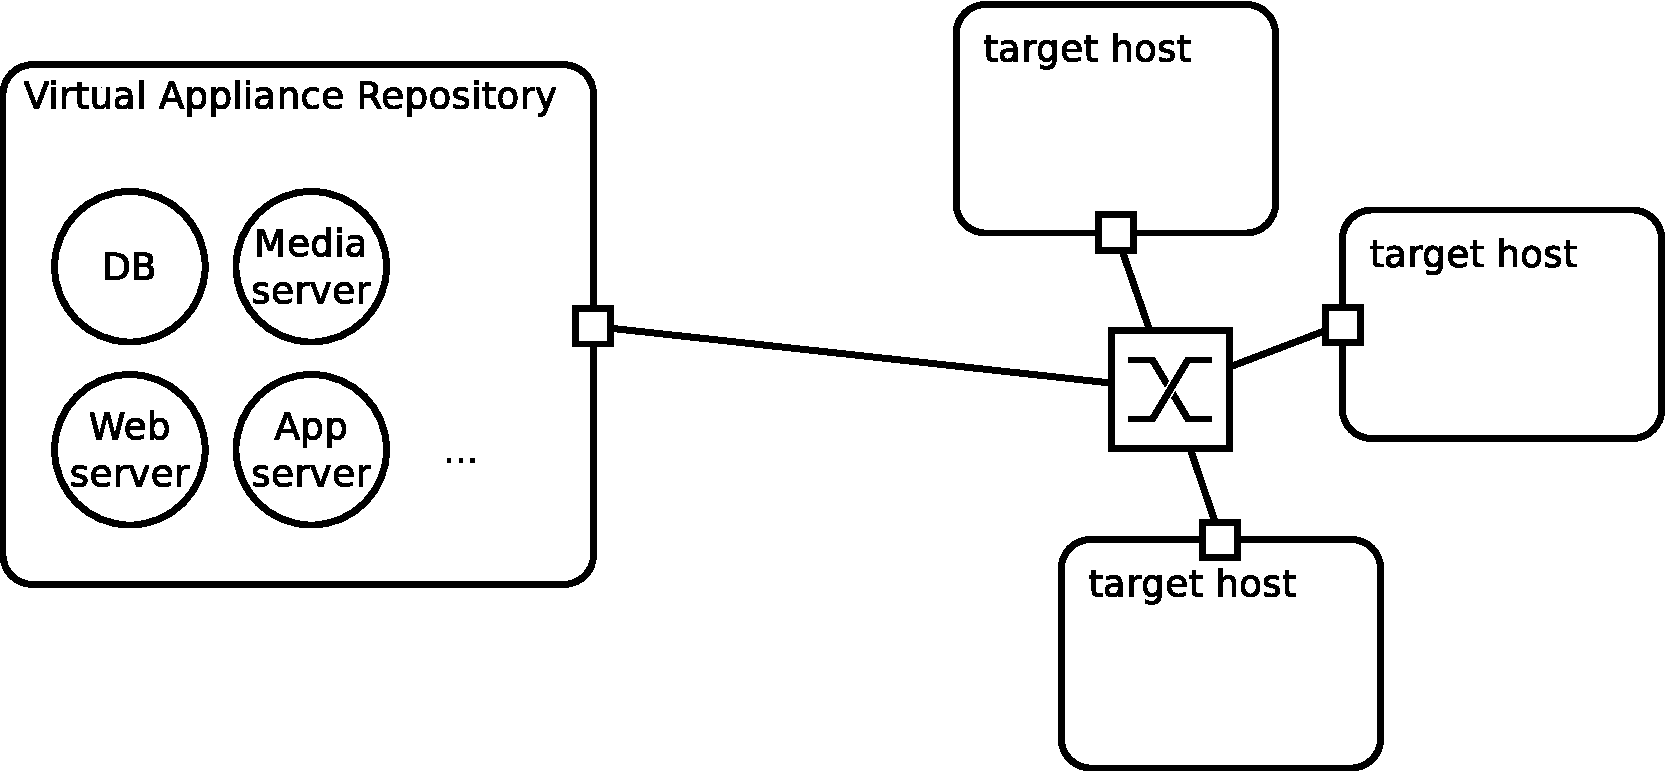
\includegraphics[width=.7\textwidth]{img/solaris/virtual-appliance-infra.pdf}
          \end{center}

          \caption{An example of infrastructure utilizing virtual appliances with appliance repository.}
        \end{figure}


    \section{Crossbow - network virtualization technology}
    \label{sec:sol:xbow}

      % TODO when introduced? +citation

      It is generally acknowledged that Crossbow was invented in China in 341 B.C but it was in middle ages when 
      it earned its recognition. Very easy in use and simultaneously very effective. The Solaris Crossbow mechanism 
      for QoS are just like real crossbows, very efficient in comparison to other existing QoS mechanisms and this
      similarity indicates the project name origin.


      \subsection{Crossbow architecture}

        One of the most important conditions in terms of network virtualization is that network traffic should be
        insulated between virtual machines. This kind of isolation can be achieved by having a dedicated physical NIC,
        network cable and port from the switch to the virtual machine itself. Moreover, switch must also ensure
        sustainability on every port. Otherwise, virtual machines will definitely interfere with each other \cite{crossbow}.
        
        In a particular case when a physical NIC has to be shared between virtual machines the most promising solution is
        to virtualize NIC hardware and the second layer of the OSI/ISO stack where sharing is fair and interference
        will be avoided. These approach was adapted in the Crossbow architecture in the Solaris OS \cite{crossbow}.
        
        Traffic separation is achieved with fundamental blocks of new architecture which are Virtual NICs (VNICs)
        created by partitioning physical NIC. A VNIC can be created over NIC or Etherstub and
        be dynamically controlled by the bandwidth and CPU resources assigned to it
        \cite{crossbow,network_virtualization}. New architecture after introducing new networking features combined with
        existing features like Solaris Containers, resource control can be presented as following:

        \begin{figure}[H]
          \begin{center}
            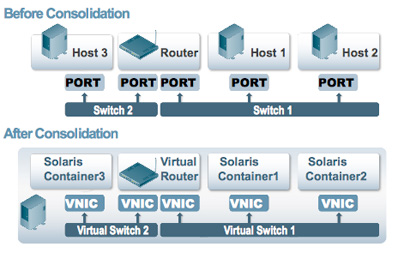
\includegraphics[width=.7\textwidth]{img/crossbow.jpg}
          \end{center}

          \caption{The Solaris Crossbow network virtualization enhancement, source: http://www.net-security.org/secworld.php?id=7573}
                  %@todo add preceise url}
        \end{figure}

        The crossbow architecture has introduced fully parallel network stack structure. Each stack could be seen as
        an independent lane (without any shared locks, queues, and CPUs) therefore network isolation is guaranteed.
        Key concept is hardware classification performed by the NIC over which VNIC was created.  Each lane has a
        dedicated buffer for Transmit (Tx) and Receive (Rx) ring. In case when load exceeds assigned limit packets must
        be dropped as it is wiser to drop them than to expend OS CPU resources \cite{crossbow}.

        \begin{figure}[H]
          \begin{center}
            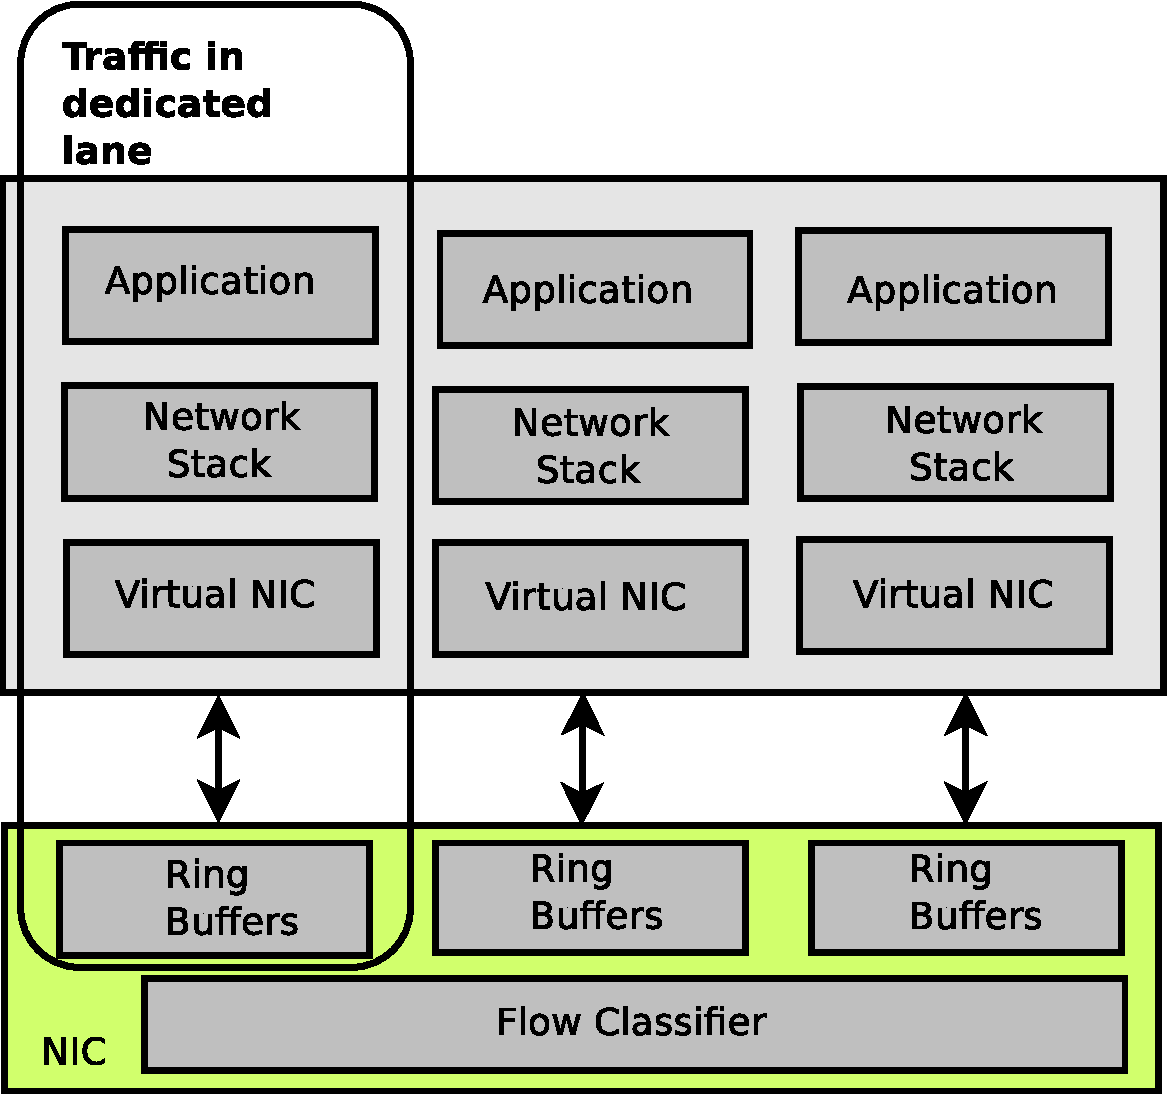
\includegraphics[width=0.5\textwidth]{img/crossbow-traffic-dedicated-line.pdf}
          \end{center}

          \caption{Dedicated lanes in the Crossbow architecture}
        \end{figure}

		
      \subsection{Virtualization lanes}

        Virtualization lane is the most key component in the Crossbow architecture. Each lane consists of some dedicated
        hardware and software that might be used to handle specific type of traffic. It usually would be composed of: 

        \begin{enumerate}
          \item NIC resources (receive and transmit rings, interrupts, MAC address slots),
          \item Driver resources (DMA bindings),
          \item MAC layer resources (data structures, execution threads, locks).
        \end{enumerate}
        
        A virtualization lane can be one of two types, hardware-based or software-based.

        
        \subsubsection{Hardware-based virtualization lanes}
        
          This type requires ability to partitioning resources from NIC. The minimum requirement is that a
          hardware-based lane should must have a dedicated receive ring.  Other resources such as transmit lane can be
          exclusive or shared between lanes. Each virtual machine could have one or more lanes assigned and the incoming
          packets would be distributed among them based on even scheduling unless some administrative polices where
          created, such as priority or bandwidth limit \cite{crossbow}.		

        
        \subsubsection{Software-based virtualization lanes}
        
          In case when NIC runs out of hardware-based virtualization lane, receive and transmit rings may be shared by
          multiple VNICs. The number of software-based virtualization lanes also often called softrings is unlimited.
          The main disadvantage of software-based lanes is the lack of fairness and isolation which in fact is provided
          in hardware-based lanes. The received and sent rings may work also in mix mode, whereas some of the rings may
          be assigned to software and some may be assigned to hardware based lanes \cite{crossbow}.	
			
      \subsection{Dynamic polling}	
        
        The Crossbow architecture proposed two types of working modes. Currently used mode is determined by traffic and
        load. Under low load, where the rate of arriving packets is lower than time of packet processing, a lane works in
        the interrupt mode which means that receive ring generates an interrupt when new packet arrives. However, when
        the backlog grows, the line switches to dynamic polling mode in which a kernel thread goes down to the receive
        ring in the NIC hardware to extract all outstanding packets in a single chain. Key aspect is that every
        virtualization lane works independently and transparently from each other. Usually only three threads are used
        per lane \cite{crossbow}:
        
        \begin{enumerate}
          \item Poll thread which goes to the NIC hardware to get all packet chain,
          \item Worker thread which is responsible for protocol processing (IP and above) or delivers packets to virtual
                machine. Thread performs also any additional transmit work which is a natural 
                requirement some concrete protocol, such as processing TCP packets that require sending ACK packets,
          \item Transmit thread that is activated when if packets are being sent after transmit side flow control relief
                discharge, or after retrieving transmit descriptor. Application or virtual 
                machine can transmit any packets without performing queuing because of flow control or context switching.
        \end{enumerate}


      \subsection{Virtual switching}
        
        Virtual switches are always created implicitly when the first VNIC is defined under existing NIC and could never
        be accessed directly nor be visible by any user (even administrator) \cite{crossbow2}. 
        
        \begin{figure}[H]
          \begin{center}
            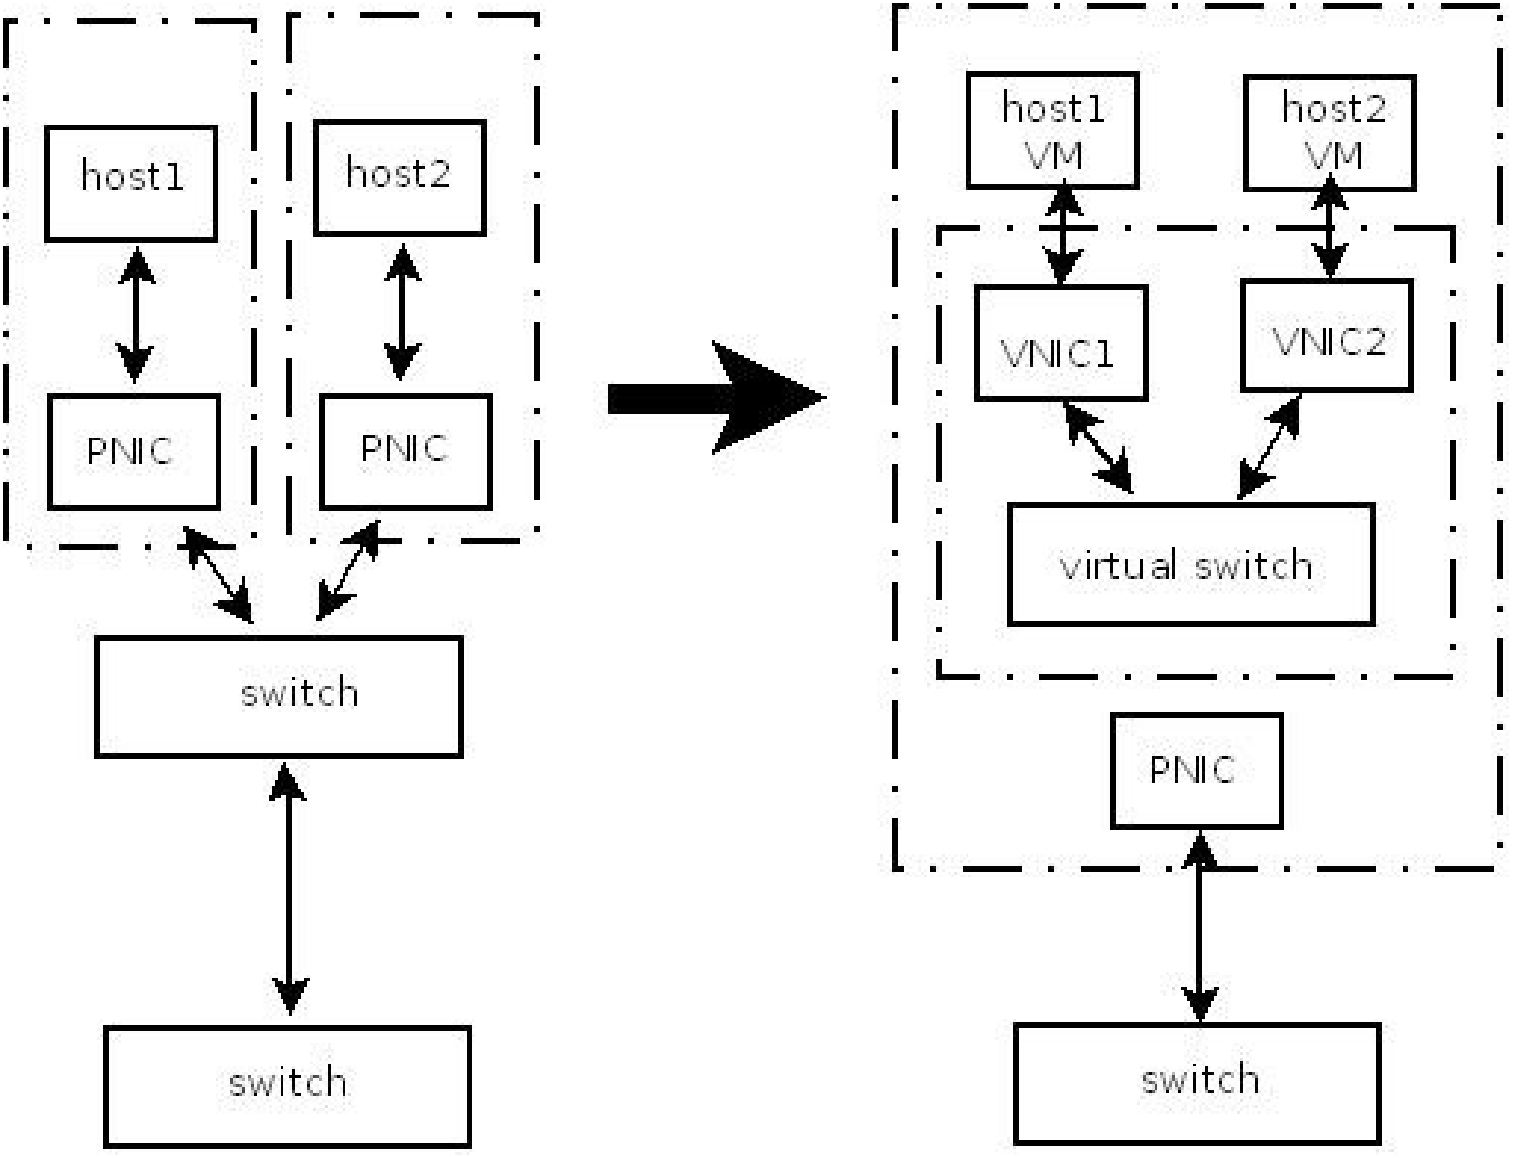
\includegraphics[width=.7\textwidth]{img/physical_and_virtual_switches_mapping.pdf}
          \end{center}

          \caption{Mapping between physical and virtual network building elements}
        \end{figure}
        
        Semantics assured by virtual switches is the same as provided by physical switches: 

        \begin{enumerate}
          \item VNICs created on top of the same NIC can send packets to each other,
          \item Broadcast packets received by the underlying NIC are distributed to every single VNIC that was defined
                on the top of this NIC,
          \item Broadcast packets sent by one of the VNICs is distributed to all VNICs defined on the top of the same
                NIC and to the NIC for further transmission as well,
          \item In terms of multicast network traffic multicast group membership is monitored and used for distributing
                packets to appropriate VNIC.
        \end{enumerate}

        Data Link Layer connectivity between VNICs is available only when they were defined on top of the same NIC. 

	
      \subsection{Crossbow components}

        The Crossbow specification describes three major components: VNICs, Etherstubs and Flows. This section gives an
        insight into their application and usage.

                
        \subsubsection{VNICs}
        
          Virtual NICs (VNICs) each containing their own lane are the key element in crossbow architecture. There is no
          difference between NIC and VNIC in administration, as they are all treated as data links. Every VNIC has an
          assigned lane and flow classifier which classifies received packets by VNIC's MAC address and sometimes by the
          VLAN tag.  If created with a VLAN tag, protocols like GVRP or MVRP may be used to register the VLAN tag with
          the physical switches too \cite{crossbow}.	

          In terms of sharing bandwidth, Crossbow enables administrative control of bandwidth for every single VNIC. The
          bandwidth of the link is implemented by regulating the periodic intake of incoming packets per dedicated lane.
          The network stack allows only as many packets as it was assigned to specific VNIC. The lane picks more packets
          when the next period begins. In case of regulating the speed of transmited bandwidth it is much easier as the
          network stack can either control the application that is generating the stream of packets or just drop the
          excessive amount of packets.  These mechanisms are also used in flows QoS described and discussed later in
          this paper \cite{crossbow}.


        \subsubsection{Etherstubs}

          As it was mentioned before, the MAC layer provides the virtual switching capabilities which allow VNICs to be
          created over existing physical NICs.  In some cases, creating virtual networks without the use of a physical
          NIC is more welcomed than creating over physical NICs. In that case VNICs would be defined on the top of
          pseudo NICs.  The Crossbow provides these kind of elements which are called Etherstubs. These components could
          be used instead of NICs during creation of VNICs \cite{crossbow}.


        \subsubsection{Flows}

          Flows are additional instruments created to allow easier network traffic administration. They might be used in
          order to provide bandwidth resource control and priority for protocols, services, containers. Virtual
          networks can be described to maintain isolation and different network properties, and define flows to manage quality
          of service \cite{network_virtualization}.

          Defined flow is a set of attributes based on Layer 3 and Layer 4 headers of the OSI/ISO model which are then
          used to identify protocol, service or virtual machine.  Flows assigned to a link must be independent therefore
          before adding new one its correctness is checked. Input and output packets are matched to flows in very
          efficient manner with minimal performance impact.

          \medskip

          Crossbow flows can be created with one of the following sets of attributes:

          \begin{itemize}
            \item Services (protocol + remote/local ports),
            \item Transport (TCP, UDP, SCTP, iSCSI, etc),
            \item IP addresses and IP subnets,
            \item DSCP field.
          \end{itemize}

          For each flow the following properties can be set \cite{flows2}: 

          \begin{itemize}
            \item bandwidth,
            \item priority.
          \end{itemize}

          \medskip

          

          \textbf{flowadm} is the console command used to create, modify, remove or to display network bandwidth and
          priority limits assigned to a particular link. 


      \subsection{Running examples of flowadm and dladm command}

        \textbf{dladm} and \textbf{flowadm} are two basic administrative commands for dealing with the Crossbow's
        components. Below a few general examples of their usage are presented.
  
        \textbf{dladm} is the admin command for crossbow datalinks elements management. Below a few examples of VNICs,
        Etherstubs management commands are presented and how bandwidth and priority values might be assigned to these
        elements.
  
        \begin{enumerate}
          \item \# dladm create-vnic vnic1 -l e1000g0 - creates new VNIC \textbf{vnic1} over existing NIC \textbf{e1000g0},
          \item \# dladm create-etherstub ether00 - creates new Etherstub \textbf{ether00},
          \item \# dladm show-linkprop vnic11 - lists all properties assigned to \textbf{vnic11} link,
          \item \# dladm set-linkprop -pmaxbw=1000 vnic11 - assignes 1Mbps bandwith limit to \textbf{vnic11} link,
          \item \# dladm set-linkprop -ppriority=low vnic11 - assignes low priority to \textbf{vnic11} link.
        \end{enumerate}
  
        More examples can be found in \textbf{man dladm}.

        \medskip

        \textbf{flowadm} is the admin command for flow management. It might be used as follows:     

        \begin{enumerate}
          \item \# flowadm show-flow -l e1000g0 - displays all flows assigned to link \textbf{e1000g0},
          \item \# flowadm add-flow -l e1000g0 -a transport=udp udpflow - creates new flow assigned to link
                \textbf{e1000g0} for all udp packets.
        \end{enumerate}

        More information about \textbf{flowadm} and \textbf{dladm} tools can be found in manual.


      \subsection{Crossbow and Differentiated Services - interoperability}
      \label{sub:sol:diffserv}

        The Crossbow technology is designed to work inside single operating system instance, there are no mechanisms
        meant to cope with problems that arise when dealing with installations spanning multiple physical machines
        connected with traditional (non-virtual) network. Crossbow's flows are, by design, relatively simple (when
        compared to DiffServ) but more efficient as far as receive performance is considered \cite{xbow-vertically}.
        Crossbow, unlike DiffServ, does not require special hardware, although if it is present it can boost overall
        operation performance \cite{xbow-vertically}.

        DiffServ, on the other hand, provides sophisticated QoS mechanisms that require proper hardware (DiffServ-aware
        routers) to be present for it to work. DiffServ is standardized (RFC 2475) and offers a multiplicity of
        classification, marking, policing and traffic shaping alternatives \cite{rfc2475}. Special fields (called DSCP)
        contained in IP packet's header are used to carry processing-related information with packets. The approach can
        be used with complex networks, comprising a number of routers with QoS awareness.

        These two environments complement one another rather than compete. Crossbow supports flow matching based on the
        DSCP field value. DSCP field generation is planned but not yet supported. It is possible (although, at the
        moment, only partially) to integrate these and build a comprehensive end-to-end networking solution with QoS
        support and virtualized components.

        \begin{figure}[H]
          \begin{center}
            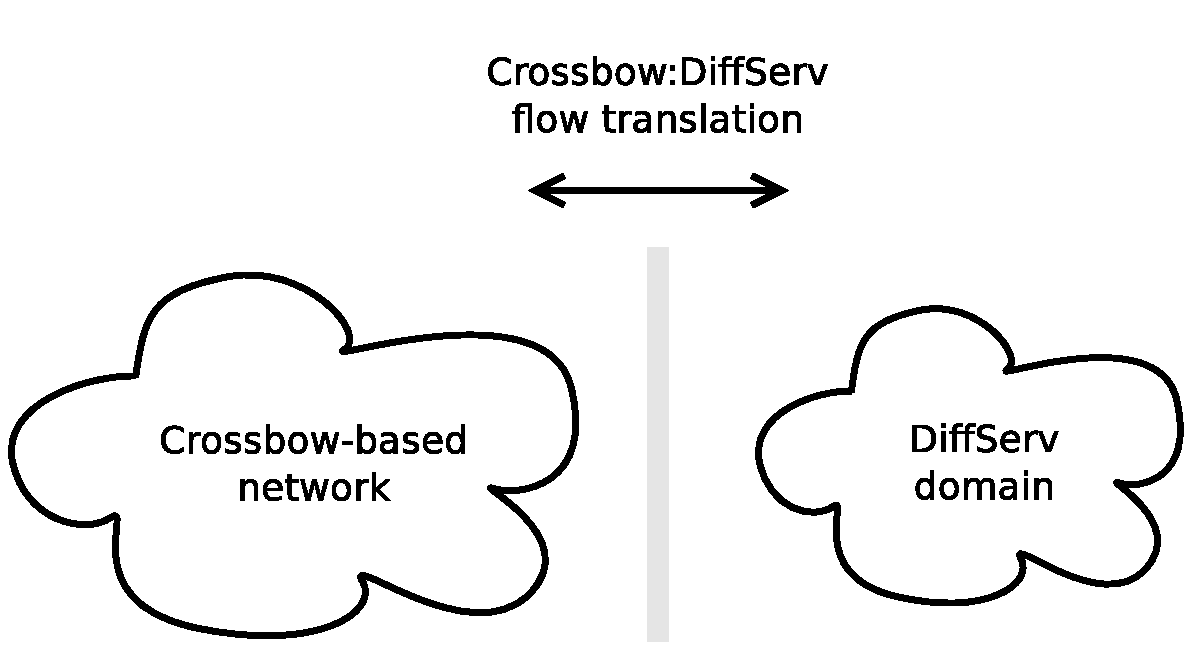
\includegraphics[width=.7\textwidth]{img/solaris/xbow-diffserv.pdf}
          \end{center}

          \caption{DiffServ integration using Crossbow-provided mechanisms}
        \end{figure}


    \section{Resource control}
    \label{sec:sol:res}

      Nowadays existing operating systems must provide mechanisms for response to the varying resource demands per
      workload which is an aggregation of processes of an application. By default resource management features are not
      used and system gives equal access to resources. When necessary, it is possible to modify this default behaviour
      with respect to different workloads. It is allowed to:

      \begin{enumerate}
        \item Restrict access to specific resource,
        \item Offer resources to workloads on a preferential basis,
        \item Isolate workloads from each another.
      \end{enumerate}
	
      Resource is any part of computing system that may be modified in order to change application behaviour. Resource
      management enables more effective resource utilization and avoid wasting available ones due to load variability.
      Reserving additional capability during off-peak periods and effective sharing resources definitely increases
      application performance.

      Most of the operating systems limited the resource control just to per-process control, whereas Oracle Solaris has
      extended this concept to the task, project and zone. Due to introducing granularity levels processes, tasks, and 
      zones are efficiently controlled from excessive resource consumption. All these enhacements are available thanks 
      to resource controls (rctls) facility \cite{oracle_admin_guide}.
      
      Solaris Operating System introduced three types of resource management control mechanisms:

      \begin{enumerate}
        \item constraints - allows defining set of bounds on used resources for a workload,
        \item partitioning - enables binding subset of system's available resources to specific workload,
        \item scheduling - involves predictable algorithm making sequence of allocation decisions at specific intervals.
      \end{enumerate}

      Hierarchical architecture allows defining set of resource control sets on each level. However, if more than one is
      assigned to a resource, the smallest container's control level is enforced \cite{oracle_admin_guide}. 

      \begin{figure}[H]
        \begin{center}
          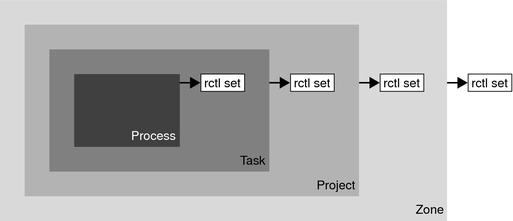
\includegraphics[width=.7\textwidth]{img/rctrl.png}
        \end{center}
        
        \caption{Solaris system multilevel architecture and its resource control sets (source: http://oracle.com)}
                          %@todo add preceise url}
		  \end{figure}


      \subsection{Accounting}
      \label{sub:sol:acct}

        Highly configurable accounting facility is provided as part of the system. Its role is to gather historical
        usage records of system and network resources. There are two levels accounting can work on in Solaris
        OS - basic and extended. Basic accounting allows for per-zone and per-project statistics gathering while
        extended accounting facility makes it possible to collect the data for tasks and processes. Statistics gathered
        by the extended accounting can be examined using C or Perl interface of the libexacct library \cite{sag}.

        The extended accounting facility can gather data for:

        \begin{itemize}
          \item system resources usage (per-task and per-process),
          \item flows defined with the IPQoS tools,
          \item links and flows created with Crossbow.
        \end{itemize}

        % TODO what data can be gathered?
                

    \section*{Summary}

      The chapter presented Solaris operating system with regard to resource virtualization. The stack of tools
      integrated into the system provides extensive support for virtualization techniques: Containers facilitate
      OS-level resource virtualization and Crossbow, shipped with Solaris 11, makes virtualization of networking
      resources possible. Resource control subsystem gives the administrator even more fine-grained control over
      resource utilization. Last, but not least, accounting functionality provides detailed view of resource usage
      history.

      The features mentioned above make realization of flexible, scalable and efficient systems possible. With these
      foundations, it is possible to build and consolidate complex network-oriented infrastructures that prove to be
      reliable, relatively easy to manage and adjust to changing requirements.

      Solaris 10 OS seems to be ideal cross-platform choice for customers dealing with management of high level
      services, complex system administration and high costs. It is the only open operating system which has proven
      results running from every critical enterprise databases to high performance Web farms that is why Solaris OS is
      becoming strategic platform for today's constantly growing demands towards operating systems \cite{solaris_operating_system}. 


  \chapter{The system architecture}

    \section*{Chapter overview}

      The \nameref{sec:domain-model} section describes the transformations performed by the system's components in order
      to instantiate/deploy an object model. These include simple one-node instantiation as well as more complex
      multi-node instantiations.

      % tutaj tez kilka slow i JIMSie i integracji + co to daje

        \begin{figure}[H]
          \begin{center}
            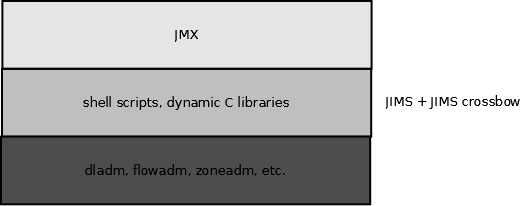
\includegraphics[width=0.8\textwidth]{img/architecture/layered_architecture.png}
          \end{center}
          \caption{Layered system architecture}
        \end{figure}  


    \section{High-level design}


    \section{System components and their responsibilities}

      \subsection{Assigner}

      \subsection{Supervisor}

      \subsection{Worker}


    \section{Crossbow resources instrumentation}


    \section{Domain model and data flows} \label{sec:domain-model}

    Created object model allows to describe network structure contaning of: switches, resources with attached addressable 
    interfaces and policies. Figure below presents concrete classes and their dependencies.    

        \begin{figure}[H]
          \begin{center}
            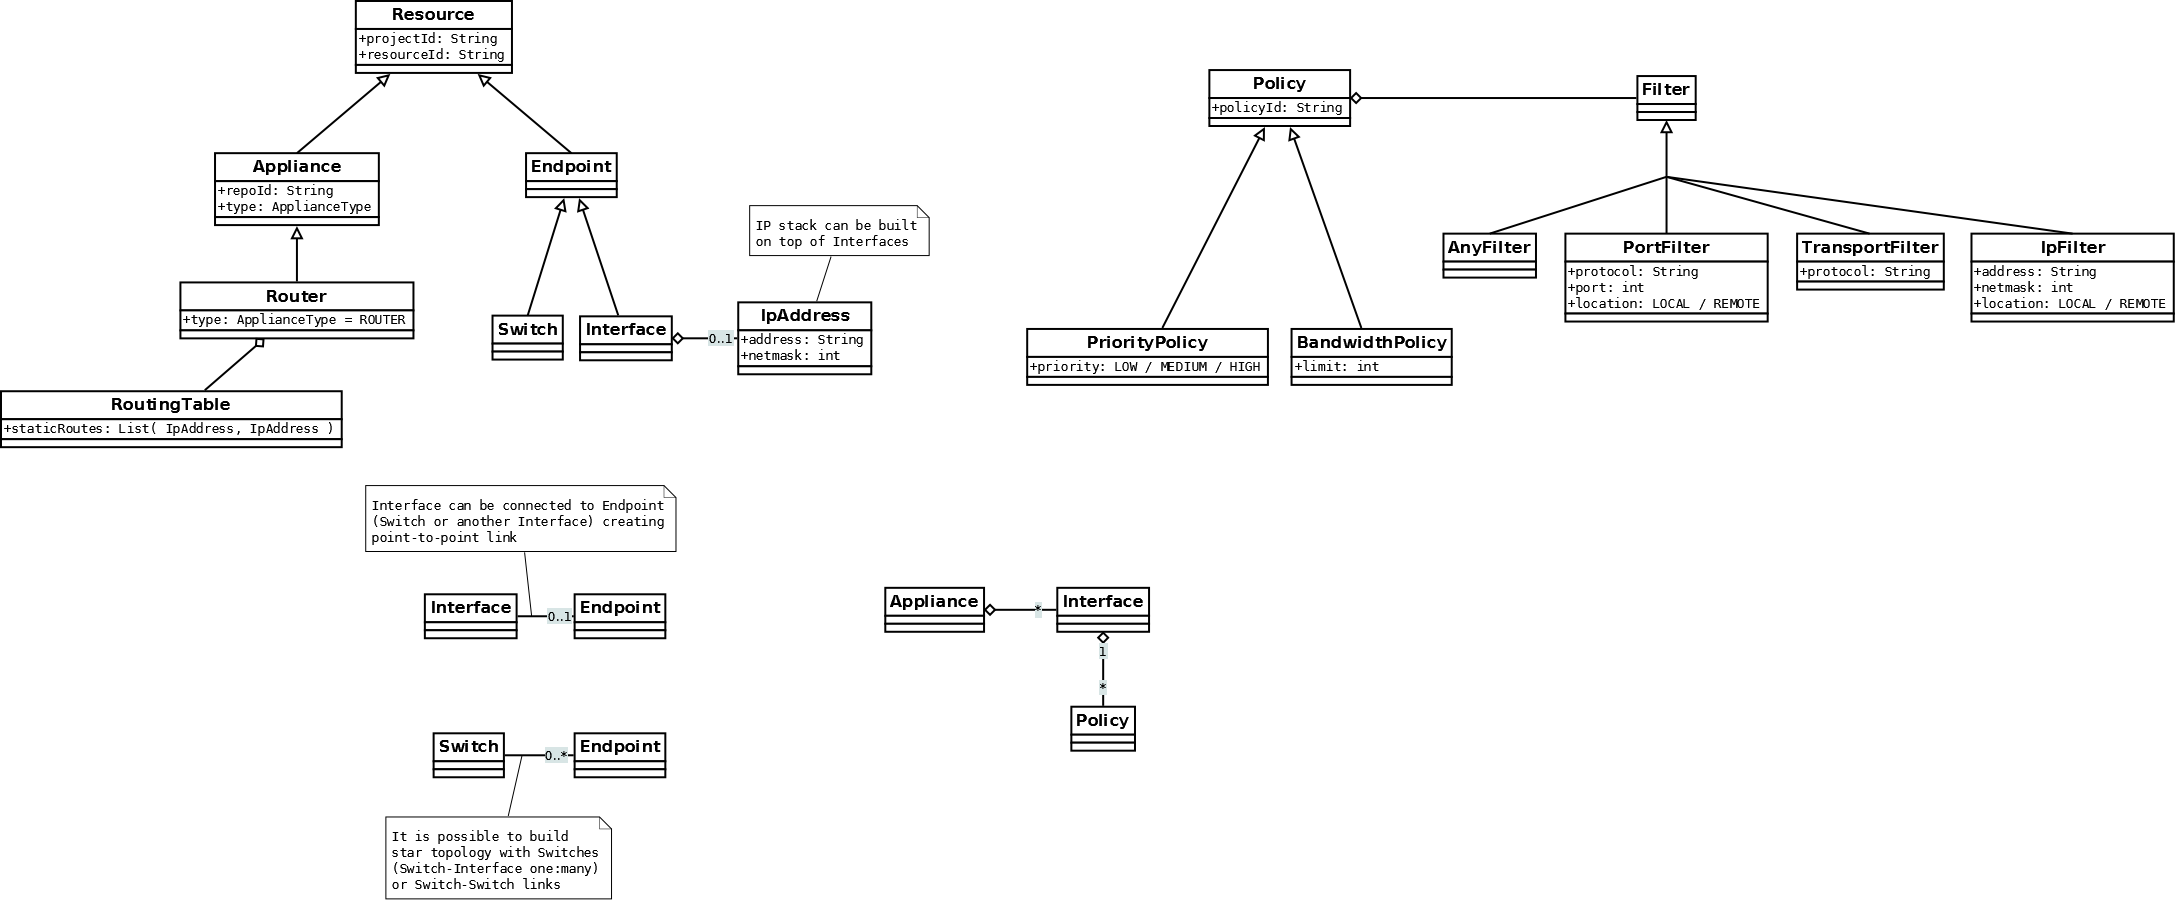
\includegraphics[angle=90, height=0.9\textwidth]{img/impl/resource-object-model.png}
          \end{center}
          \caption{Resource object model and their relationships}
        \end{figure}        


    \section*{Summary}


  \chapter{Implementation}
    
    \section*{Chapter overview}


    \section{Implementation environment}

    \section{Crossbow components implementational details}

        %TODO czy tutaj te diagramy pasuja???

        \begin{figure}[H]
          \begin{center}
            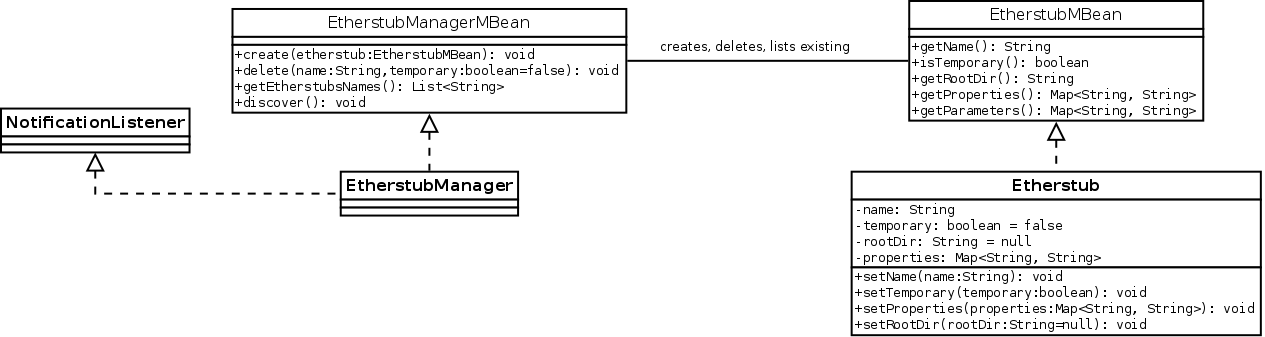
\includegraphics[width=0.8\textwidth]{img/impl/etherstub.png}
          \end{center}
          \caption{Etherstub class diagram}
        \end{figure}        

        \begin{figure}[H]
          \begin{center}
            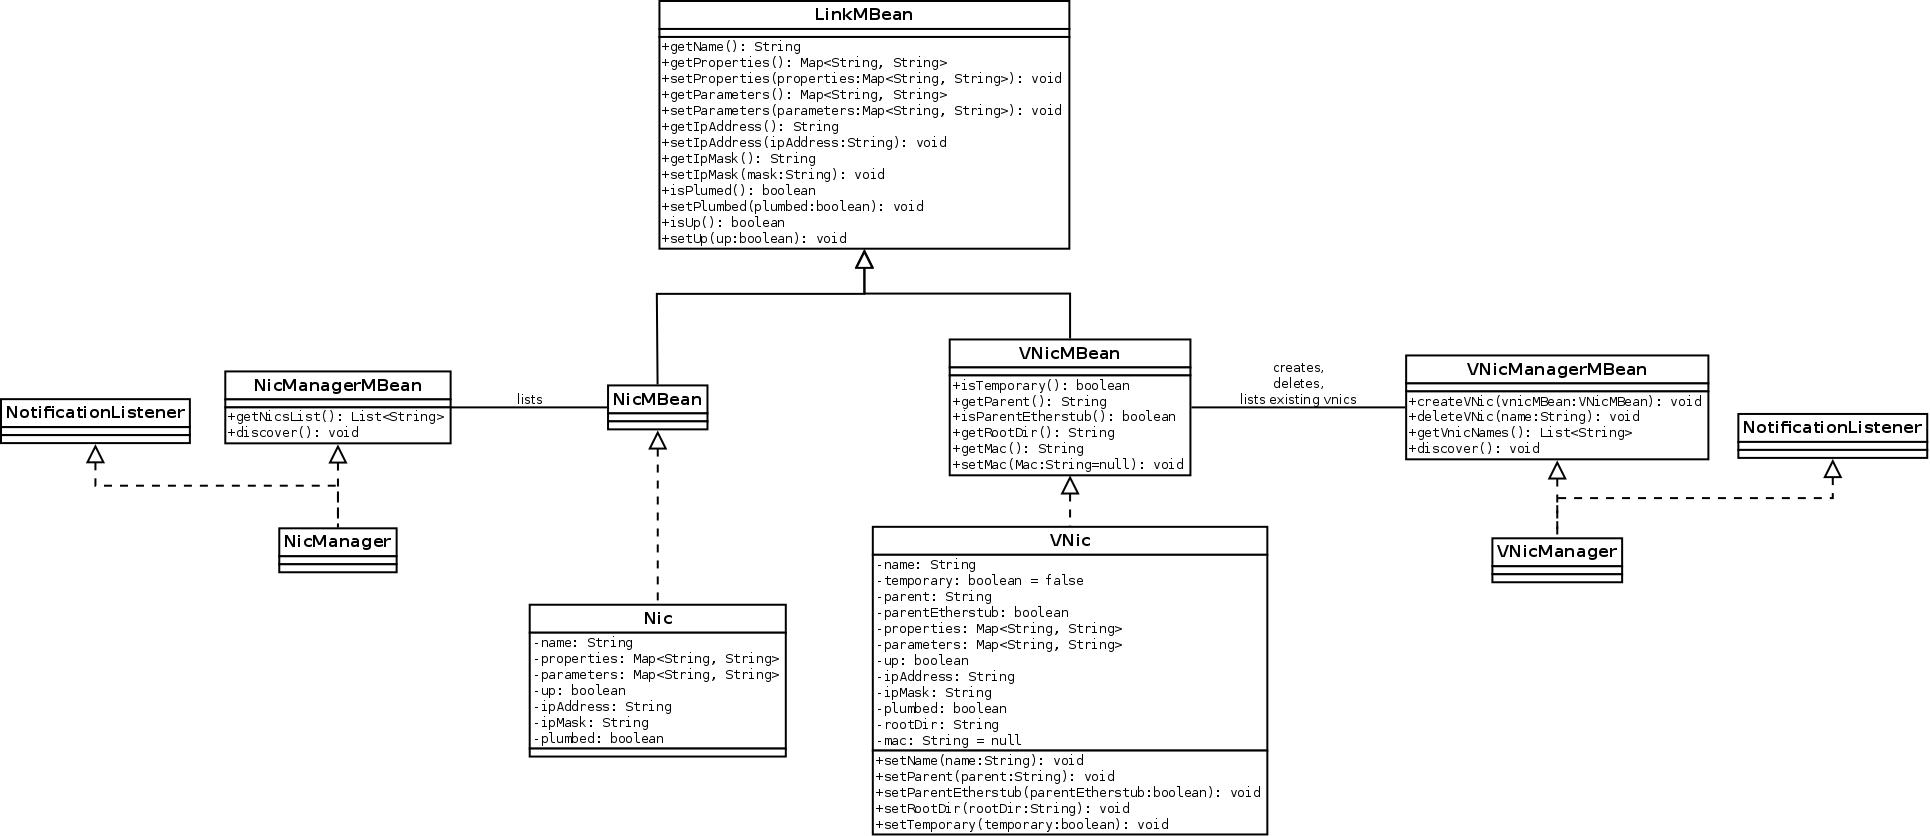
\includegraphics[width=0.8\textwidth]{img/impl/link.png}
          \end{center}
          \caption{Link (VNic, Nic) class diagram}
        \end{figure}        

        \begin{figure}[H]
          \begin{center}
            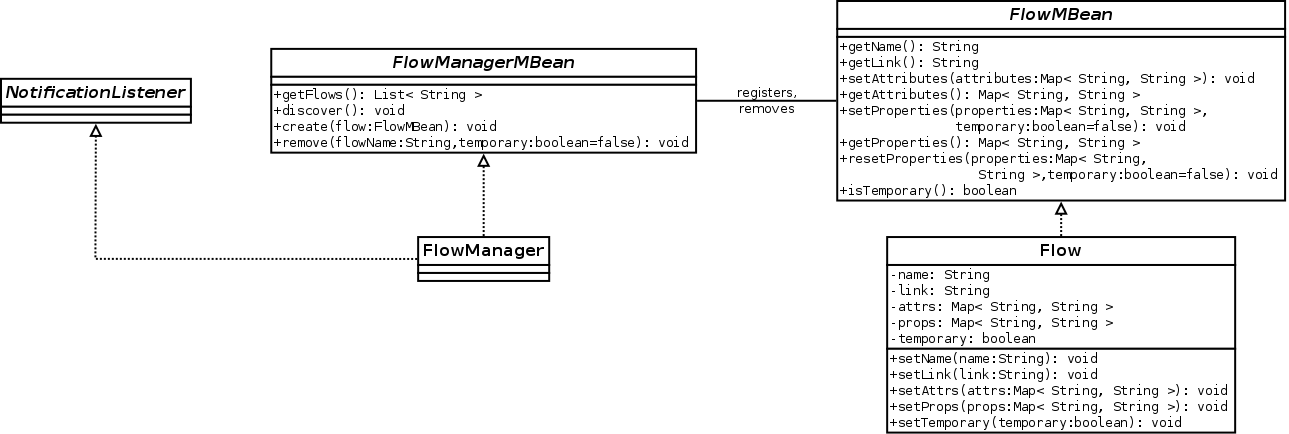
\includegraphics[width=0.8\textwidth]{img/impl/flow.png}
          \end{center}
          \caption{Flow class diagram}
        \end{figure}        

        


    \section{Domain model transformation details}
        


    \section{Low-level functions access}


    \section{Building and running the platform}


    \section*{Summary}


  \chapter{Case Study}

    The chapter describes experimental studies.

    \section{Multimedia server}

      \subsection{Scenario description}

        % TODO
        %
        % * DSS VA
        % * mplayer na VA klienckich
        % * tshark

        % na kazdej zonce tshark i zbieranie danych do pcap
        % analiza+wykresy (jitter, opuszczone pakiety) - wireshark
        % serwer - darwin
        % klient - mplayer


        \begin{itemize}
          \item similar to DiffServ (traffic classes, selectors, filters, priority, queuing)
          \item DiffServ doesn't specify anything virtual
          \item DSS and adaptive codecs
        \end{itemize}

        \begin{itemize}
          \item 2 classes: VOD + streaming
          \item \_ unicast \_ vs multicast streaming
          \item access rules for resources of different quality
          \item enabling QoS for defined classes
          \item priorities + limiting the bandwidth (per user)!
          \item 3 users: 2 streaming, 1 VOD
        \end{itemize}

        \begin{figure}[H]
          \begin{center}
            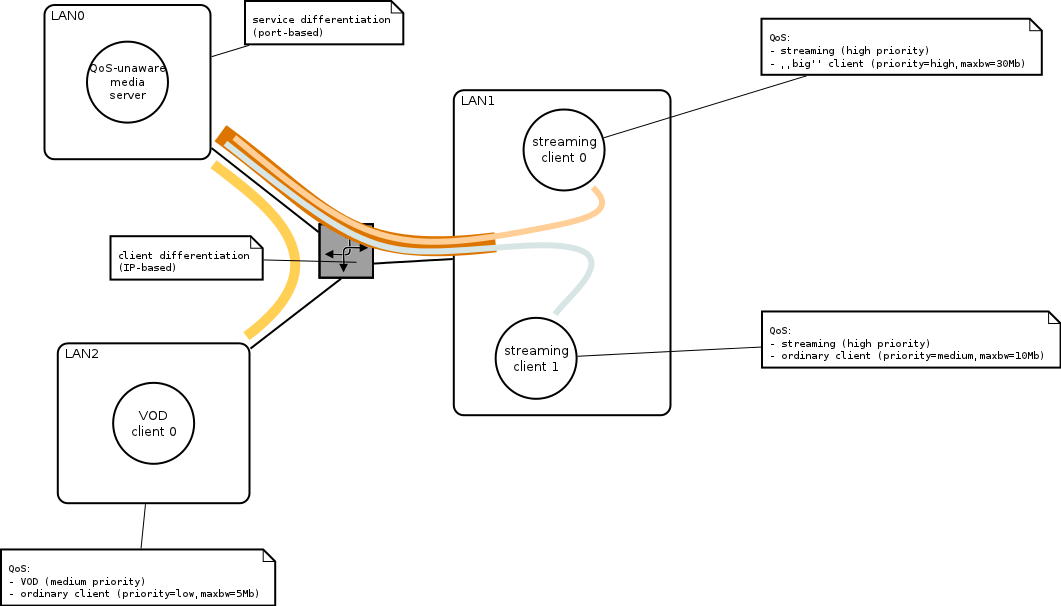
\includegraphics[width=0.8\textwidth]{img/test-case/diagram.png}
          \end{center}

          \caption{VOD + streaming clients test case example}
        \end{figure}


      \subsection{Resource access requirements}

      \subsection{Providing tunable and scalable virtual infrastructure}


    \section*{Summary}


  \chapter{Summary}

    \section*{Chapter overview}

      Bibliography \cite{mittelbach2004} test.
	
		

    \section{Conclusions}
	
		

    \section{Achieved goals}
	
		

    \section{Further work}
	
	In terms of the future work there are many improvements that might be implemented. Probably the largest component, which was initially plannned to be implemented, was automatic resource assigner, that would run
        and perform automatic resource assignments to nodes that run under lowest load. This assigner with attached rule based system would gather data about the load on each node and based on that 
	decide what and where instantiate. Presented and discussed system in this thesis lacks that functionality. Instead, it offers manual assignments, where user must select on which node his virtual resources should be created. 


  \bibliographystyle{plain}
  \bibliography{bibliography}


\end{document}

% vim: et : tw=120 : spelllang=en_us,pl : spell :
